\documentclass{article}
\usepackage{graphicx}
\usepackage{epsfig}
%\usepackage{caption}
%\usepackage{subcaption}
\usepackage{epsf}
\usepackage{amssymb}
\usepackage{epstopdf}
\usepackage{amsmath}
\usepackage{braket}
\usepackage{multirow}
\usepackage{array}
\usepackage{mathrsfs}

\makeatletter
\renewcommand{\fnum@figure}{Fig. \thefigure}
\makeatother

\begin{document}

\title{Dipole-Dipole/Cavity-Cavity interaction in the Squeezed Vacuum}
\maketitle 




\section{Three Level Atom}
In this section, we consider a scenario where a three-level atom is located inside the waveguide with the squeezed vacuum injected from both ends, as shown in Fig.~\ref{1}(a). The atomic electronic structure is shown in Fig.~\ref{1}(b) where the atomic states are labeled $|a\rangle$, $|b\rangle$, $|c\rangle$ from the excited state to the ground state. We assume that $\omega_{ac}=2\omega_0$ where $\omega_0$ is the center frequency of the broad band squeed vacuum. $\omega_{ab}$ and $\omega_{bc}$ are not equal but they are still within the bandwith of the squeezed vacuum.  
\begin{figure*}
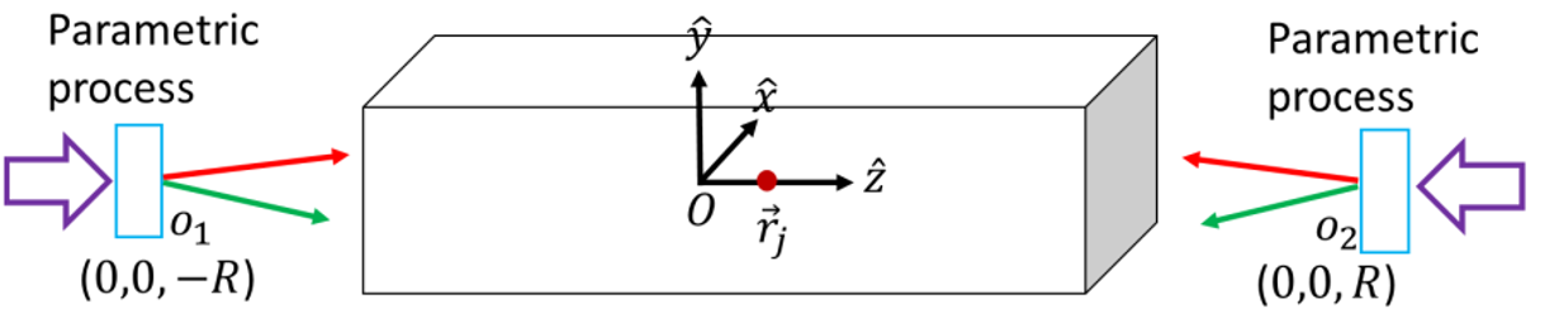
\includegraphics[width=0.7\columnwidth]{fig1.png}
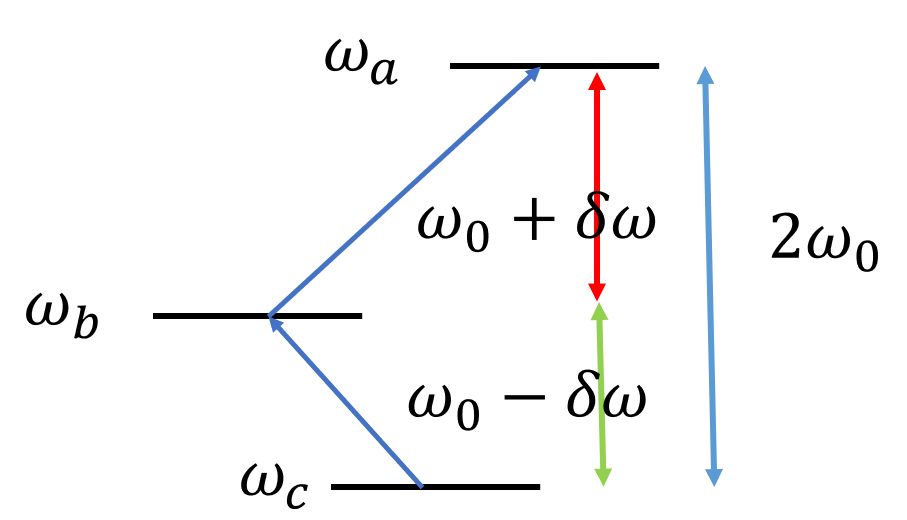
\includegraphics[width=0.25\columnwidth]{fig2.png}
\caption{(a) Schematic setup: A three-level atom is located inside the waveguide with the broadband squeezed vacuum incident from both ends. (b)The energy structure of the three level atom. Transition $|a\rangle\rightarrow|c\rangle$ is forbidden and $\omega_{ac}=2\omega_0$ where $\omega_0$ is the center frequency of the squeezed vacuum. $\omega_{ab}$ and $\omega_{bc}$ differ by a small amount $2\delta\omega_0$ and they are within the bandwidth of the squeezed vacuum reservoir.}
\label{1}
\end{figure*}

The general master equation of dipole-dipole interaction in the squeezed vacuum can be used to study the dynamics of the three-level atom\cite{You2018}:
\begin{equation}
\label{eq1}
\begin{split}
\frac{d\rho^{S}}{dt}=&-i\underset{i\neq j}{\sum}\Lambda_{ij}[S_{i}^{+}S_{j}^{-},\rho^{S}]e^{i(\omega_{i}-\omega_{j})t}\\
&-\frac{1}{2}\underset{i,j}{\sum}\gamma{}_{ij}(1+N)(\rho^{S}S_{i}^{+}S_{j}^{-}+S_{i}^{+}S_{j}^{-}\rho^{S}-2S_{j}^{-}\rho^{S}S_{i}^{+})e^{i(\omega_{i}-\omega_{j})t} \\
&-\frac{1}{2}\underset{i,j}{\sum}\gamma{}_{ij}N(\rho^{S}S_{i}^{-}S_{j}^{+}+S_{i}^{-}S_{j}^{+}\rho^{S}-2S_{j}^{+}\rho^{S}S_{i}^{-})e^{-i(\omega_{i}-\omega_{j})t}\\
&-\frac{1}{2}\sum_{\alpha=\pm}\underset{i,j}{\sum}\gamma'_{ij}Me^{2\alpha ik_{0z}R}e^{i\alpha(\omega_i+\omega_j-2\omega_0)t}(\rho^{S}S_{i}^{\alpha}S_{j}^{\alpha}+S_{i}^{\alpha}S_{j}^{\alpha}\rho^{S}-2S_{j}^{\alpha}\rho^{S}S_{i}^{\alpha})
\end{split}
\end{equation}
where the coefficients are
\begin{equation}
\label{eq2}
\begin{split}
& \gamma_{ij}=\sqrt{\gamma_{i}\gamma_{j}}\cos(k_{0z}r_{ij}) \\
& \Lambda_{ij}=\frac{\sqrt{\gamma_{i}\gamma_{j}}}{2}\sin(k_{0z}r_{ij})\\
& \gamma'_{ij}=\sqrt{\gamma_{i}\gamma_{j}}\cos[k_{0z}(r_{i}+r_{j})]
\end{split}
\end{equation}
where $\gamma_{i}$ is the decay rate for transition $i$ in ordinary vacuum. For a single three level atom, we have $r_i=r_j$, for simplicity we set $R=r_i=0$ and $\gamma_1=\gamma_2=\gamma$. After applying the rotating wave approximation(RWA), the master equation Eq.\eqref{eq1} becomes (see Appendix A)
\begin{equation}
\label{eq3}
\begin{split}
\frac{d\rho^{S}}{dt}=&-\frac{1}{2}\underset{i}{\sum}\gamma(1+N)(\rho^{S}S_{i}^{+}S_{i}^{-}+S_{i}^{+}S_{i}^{-}\rho^{S}-2S_{i}^{-}\rho^{S}S_{i}^{+})\\
&-\frac{1}{2}\underset{i}{\sum}\gamma N(\rho^{S}S_{i}^{-}S_{i}^{+}+S_{i}^{-}S_{i}^{+}\rho^{S}-2S_{i}^{+}\rho^{S}S_{i}^{-})\\
&-\frac{1}{2}\sum_{\alpha=\pm}\underset{i\ne j}{\sum}\gamma M(\rho^{S}S_{i}^{\alpha}S_{j}^{\alpha}+S_{i}^{\alpha}S_{j}^{\alpha}\rho^{S}-2S_{j}^{\alpha}\rho^{S}S_{i}^{\alpha})
\end{split}
\end{equation}
where $N=\sinh(r)^2$ and $M=\sinh(r)\cosh(r)$The steady state of Eq.\eqref{eq3} can be derived by re-writing Eq.\eqref{eq3} as:
\begin{subequations}
\begin{align}
&\dot{\rho}_{aa}/\gamma=-ch^{2}\rho_{aa}+sh{}^{2}\rho_{bb}-\frac{1}{2}chsh(\rho_{ac}+\rho_{ca})\label{4a} \\
& \dot{\rho}_{bb}/\gamma=(ch^{2}\rho_{aa}-sh^{2}\rho_{bb})+(sh^{2}\rho_{cc}-ch^{2}\rho_{bb})+chsh(\rho_{ac}+\rho_{ca})\label{4b}\\
&\dot{\rho}_{cc}/\gamma=ch^{2}\rho_{bb}-sh^{2}\rho_{cc}-\frac{1}{2}chsh(\rho_{ac}+\rho_{ca})\label{4c}\\
&(\dot{\rho}_{ac}+\dot{\rho}_{ca})/\gamma=-\frac{1}{2}(ch^{2}+sh^{2})(\rho_{ac}+\rho_{ca})-shch(\rho_{aa}-2\rho_{bb}+\rho_{cc})\label{4d}\\
&\dot{\rho}_{ab}/\gamma=-(1+\frac{3}{2}sh^{2})\rho_{ab}-\frac{1}{2}chsh\rho_{cb}\label{4e}\\
&\dot{\rho}_{cb}/\gamma=-\frac{1}{2}chsh\rho_{ab}-(\frac{1}{2}+\frac{3}{2}sh^{2})\rho_{cb}\label{4f}
\end{align}
\end{subequations}
where $sh=\sinh(r), ch=\cosh(r)$. Eq.\eqref{4e}\eqref{4f} yield $\rho_{ab}=\rho_{cb}=0$ for the steady state, and Eq.\eqref{4a}-\eqref{4d} yield $\rho_{aa}=\frac{sh^{2}}{sh^{2}+ch^{2}}$, $\rho_{cc}=\frac{ch^{2}}{sh^{2}+ch^{2}}$, $\rho_{ac}=-\frac{shch}{sh^{2}+ch^{2}}$. Thus, the steady state is actually a superposition state of $|a\rangle$ and $|c\rangle$: $\frac{sh}{\sqrt{sh^{2}+ch^{2}}}|a\rangle-\frac{ch}{\sqrt{sh^{2}+ch^{2}}}|c\rangle$. This phenomenon is similar to coherent trapping, but here we achieve the trapping for $\Xi$ structure with the squeezed vacuum reservoir, which cannot be realized with coherent pump due to spontaneous emission.

In general we can study the steady state population distribution when the dipole moments of transition $|a\rangle\rightarrow|b\rangle$ and $|b\rangle\rightarrow|c\rangle$ are different, i.e., $\mu_{ab}\ne\mu_{bc}$. Although the analytical solution is quite lengthy, we can easily get the numerical solution for different $\mu_{ab}$ and $\mu_{bc}$. In Fig.~\ref{2}(a), population inversion is achieved with $\mu_{ab}<\mu_{bc}$. This can be interpreted with the help of Fig.~\ref{2}(c). Figure ~\ref{2}(c) shows that the direct transition between $|a\rangle$, $|b\rangle$, and $|c\rangle$ are allowed just like the thermal reservoir case. However, in the squeezed vacuum, there is additional paths for population flow: electrons in any of these three states can evolve into the other two through an intermediate "state" $\rho_{ac}$. Although $\rho_{ac}$ is actually not a state, and $\rho_{ac}<0$ in our convention, it can be used to elucidate our idea. When $\mu_{ab}\ll\mu_{bc}$, the transition $|a\rangle\rightarrow|b\rangle$ can be removed. Thus state $|c\rangle$ can be excited to $|a\rangle$ through $|c\rangle\rightarrow|b\rangle\rightarrow\rho_{ac}\rightarrow|a\rangle$, but $|a\rangle$ can not decay back to $|c\rangle$. Thus, the population is trapped from $|c\rangle$ to $|a\rangle$. Although the population inversion between $|a\rangle$ and $|c\rangle$ is very sensitive to the value of $M$, the population inversion between $|a\rangle$ and $|b\rangle$ still holds for $M=0.8\sqrt{N(N+1)}$, which is shown in Fig.~\ref{2}(b).

\begin{figure*}
\includegraphics[width=0.48\columnwidth]{atom_fig4.eps}
\includegraphics[width=0.48\columnwidth]{atom_fig5.eps}
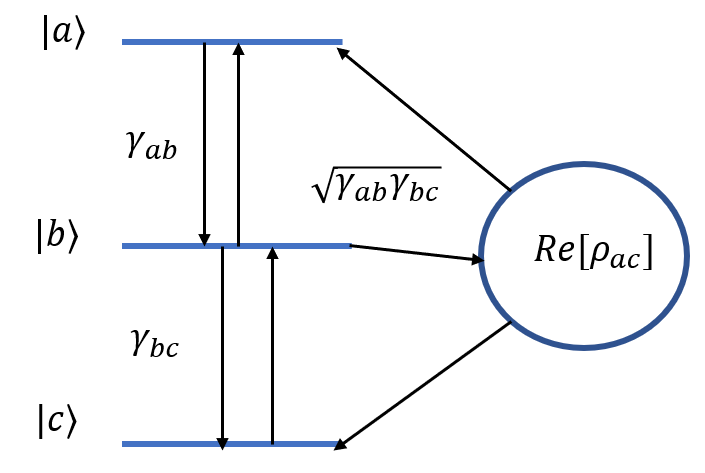
\includegraphics[width=0.4\columnwidth]{atom_fig3.png}
\caption{(a) The steady state population distribution for different $\mu_{ab}$ and$\mu_{bc}$. The squeezing parameter $r=1$. (b) The steady state population distribution for non-ideal squeezed vacuum which is characterized by the ratio of $M$ and $\sqrt{N(N+1)}$. (c) The allowed population flow in the squeezed vacuum. The squeezing parameter $r=1$, and $\mu_{ab}=\frac{1}{4}\mu_{bc}$.}
\label{2}
\end{figure*}
%\begin{equation}
%\label{eq4}
%\begin{split}
%\frac{d\rho^{S}}{dt}=&\sum_{i\ne j}\frac{\gamma}{2}[-\rho(\cosh rS_{i}^{\dagger}+\sinh rS_{j})(\cosh rS_{i}+\sinh rS_{j}^{\dagger})\\
%&-(\cosh rS_{i}^{\dagger}+\sinh rS_{j})(\cosh rS_{i}+\sinh rS_{j}^{\dagger})\rho\\
%&+2(\cosh rS_{i}+\sinh rS_{j}^{\dagger})\rho(\cosh rS_{i}^{\dagger}+\sinh rS_{j})]
%\end{split}
%\end{equation}


\section{Cavity-Cavity interaction}
In this section, we consider a similar scenario but now the atoms are replaced with single mode cavity. The schematic setup is shown in Fig.~ref{3}. The total Hamiltonian is:
\begin{equation}
\label{eq5}
\begin{split}
H=\sum_{i}\hbar\omega(a^{\dagger}a_{i}+\frac{1}{2})+\hbar\sum_{i,k}\omega_{k}(a_{i}^{\dagger}a_{i}+\frac{1}{2})+\hbar\sum_{i,k}g_{k}(a_{i}^{\dagger}a_{k}+H.c.)
\end{split}
\end{equation}
where $a_k$ stands for the mods in the waveguide and $a$ is the field operator of the single mode inside the cavity. The waveguide is saturated with the squeezed vacuum with the center frequency $\omega_0$. 


\begin{figure*}
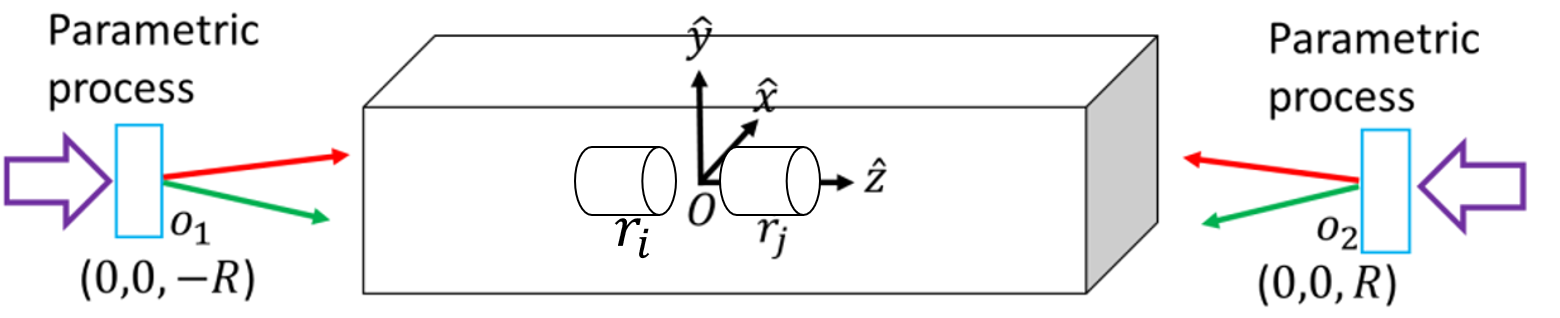
\includegraphics[width=0.8\columnwidth]{fig3.png}
\caption{(a) Schematic setup: two single-mode cavities are placed inside the waveguide with the broadband squeezed vacuum incident from both ends.}
\label{3}
\end{figure*}

First, we study two non-resonant cavities coupled to the squeezed vacuum reservoir. The eigen frequencies of these two cavities are $\omega_1=\omega_0-\delta \omega$ and $\omega_2=\omega_0+\delta \omega$, following exacly the same steps as the derivation of Eq.\eqref{eq1}, we get:
\begin{equation}
\label{eq6}
\begin{split}
\dot{\rho}&=\sum_{i}\gamma(1+N)(-\rho a_{i}^{\dagger}a_{i}-a_{i}^{\dagger}a_{i}\rho+2a_{i}\rho a_{i}^{\dagger})\\
&+\gamma N(-\rho a_{i}a_{i}^{\dagger}-a_{i}a_{i}^{\dagger}\rho+2a_{i}^{\dagger}\rho a_{i})\\
&+\sum_{i\ne j}\gamma M(e^{i(\theta_i+\theta_j)}\rho a_{i}a_{j}+e^{i(\theta_i+\theta_j)}a_{i}a_{j}\rho-2e^{i(\theta_i+\theta_j)}a_{i}\rho a_{j}+h.c.)\\
\end{split}
\end{equation}
where $\theta_i$ is a phase factor which depends on the relative position of cavities and the squeezing source. The above equation can be re-arranged as:
\begin{equation}
\label{eq7}
\begin{split}
\dot{\rho}&=\sum_{i\ne j}\frac{\gamma}{2}[-\rho(\cosh ra_{i}^{\dagger}-e^{i\theta}\sinh ra_{j})(\cosh ra_{i}-e^{-i\theta}\sinh ra_{j}^{\dagger})\\
&-(\cosh ra_{i}^{\dagger}-e^{i\theta}\sinh ra_{j})(\cosh ra_{i}-e^{-i\theta}\sinh ra_{j}^{\dagger})\rho\\
&+2(\cosh ra_{i}-e^{-i\theta}\sinh ra_{j}^{\dagger})\rho(\cosh ra_{i}^{\dagger}-e^{i\theta}\sinh ra_{j})]\\
\end{split}
\end{equation}
we use the following Bogoliubov transformation\cite{Bogoliubov}:
\begin{equation}
\label{eq8}
\begin{split}
&S=exp(\eta^{\star}a_{i}a_{j}-\eta a_{i}^{\dagger}a_{j}^{\dagger})\\
&A_{i}=S^{+}a_{i}S=\cosh(r)a_{i}-e^{-i\theta}\sinh(r)a_{j}^{\dagger} \\
&A_{i}^{+}=S^{+}a_{i}^{+}S=\cosh(r)a_{i}^{+}-e^{i\theta}\sinh(r)a_{j}\\
\end{split}
\end{equation}
so the master equation Eq.\eqref{eq7} becomes:
\begin{equation}
\label{eq9}
\begin{split}
\dot{\rho}=\sum_{i}\gamma[-\rho A_{i}^{\dagger}A_{i}-A_{i}^{\dagger}A_{i}\rho+2A_{i}\rho A_{i}^{\dagger}]
\end{split}
\end{equation}
Next we redefine the density matrix: $\rho_{s}=S\rho S^{\dagger}$. Thus Eq.\eqref{eq9} becomes:
\begin{equation}
\label{eq11}
\begin{split}
\dot{\rho}_{s}&=\sum_{i}\gamma[-\rho_{s}a_{i}^{\dagger}a_{i}-a_{i}^{\dagger}a_{i}\rho_{s}+2a_{i}\rho_{s}a_{i}^{\dagger}]\\
&\equiv\sum_{i}\gamma[-a_{i}^{l\dagger}a_{i}^{l}\rho_{s}-a_{i}^{r\dagger}a_{i}^{r}\rho_{s}+2a_{i}^{r}a_{i}^{l\dagger}\rho_{s}]\equiv L\rho_{s}
\end{split}
\end{equation}
Here we define superoperator $\{a_{i}^{l}, a_{i}^{l\dagger}\}$($\{a_{i}^{r}, a_{r}^{l\dagger}\}$ ) only acting to the left(right) on density operator $\rho$ \cite{Wang2002, An}. These operators have the following commutation relations: 
\begin{equation}
\label{eq12}
\begin{split}
[a_{i}^{r},a_{j}^{r\dagger}]=\delta_{ij},\,[a_{i}^{l},a_{j}^{l\dagger}]=-\delta_{ij},\,[a_{i}^{l},a_{j}^{r\dagger}]=[a_{i}^{l},a_{j}^{r}]=[a_{i}^{l\dagger},a_{j}^{r}]=[a_{i}^{l\dagger},a_{j}^{r\dagger}]=0
\end{split}
\end{equation}
Thus, the steady state of Eq.\eqref{eq11} can be solved by solving $L\rho=0$, which requires the diagnolization of superoperator $L$. Applying the similarity transformation $U=e^{-a_{1}^{r}a_{1}^{l\dagger}-a_{2}^{r}a_{2}^{l\dagger}}$ to Eq.\eqref{eq11} , since we have $U^{-1}(a_{i}^{r\dagger},a_{i}^{l},a_{i}^{r},a_{i}^{l\dagger})U=(a_{i}^{r\dagger}+a_{i}^{l\dagger},a_{i}^{r}+a_{i}^{l},a_{i}^{r},a_{i}^{l\dagger})$, the right hand side of Eq.\eqref{eq11} becomes:
\begin{equation}
\label{eq13}
\begin{split}
RHS=\sum_{i}\gamma U^{-1}[-a_{i}^{l\dagger}a_{i}^{l}-a_{i}^{r\dagger}a_{i}^{r}+2a_{i}^{r}a_{i}^{l\dagger}]UU^{-1}\rho_{s}=\sum_{i}\gamma[-a_{i}^{l\dagger}a_{i}^{l}-a_{i}^{r\dagger}a_{i}^{r}]U^{-1}\rho_{s}
\end{split}
\end{equation}
The only solution to $L\rho=0$ is $U^{-1}\rho_{s}=|0,0\rangle\langle0,0|$, which yields $\rho=S^{\dagger}\rho_S S=S^{\dagger}e^{-K_{-1}-K_{-2}}|0,0\rangle\langle0,0|S=S^{\dagger}|0,0\rangle\langle0,0|S$ which is the two mode squeezed vacuum.

Then we study the case where two cavities are identical, i.e., $\omega_1=\omega_2=\omega_0$. Then the master equation becomes:
\begin{equation}
\label{eq13}
\begin{split}
\dot{\rho}&=\sum_{ij}\gamma\cosh^{2}r(-\rho a_{i}^{\dagger}a_{j}-a_{i}^{\dagger}a_{j}\rho+2a_{i}\rho a_{j}^{\dagger})\\
&+\gamma\sinh^{2}r(-\rho a_{i}a_{j}^{\dagger}-a_{i}a_{j}^{\dagger}\rho+2a_{i}^{\dagger}\rho a_{j})\\
&+\gamma\cosh r\sinh r(e^{i(\theta_{i}+\theta_{j})}\rho a_{i}a_{j}+e^{i\theta}a_{i}a_{j}\rho-e^{i\theta}2a_{i}\rho a_{j}+h.c.)\\
\end{split}
\end{equation}
This equation can be rearranged when $\theta_1=\theta_2=\theta$:
\begin{equation}
\label{eq14}
\begin{split}
\dot{\rho}&=\sum_{ij}\gamma[-\rho(\cosh ra_{i}^{\dagger}-e^{i\theta}\sinh ra_{i})(\cosh ra_{j}-e^{-i\theta}\sinh ra_{j}^{\dagger})\\
&-(\cosh ra_{i}^{\dagger}-e^{i\theta}\sinh ra_{i})(\cosh ra_{j}-e^{-i\theta}\sinh ra_{j}^{\dagger})\rho\\
&+2(\cosh ra_{j}-e^{-i\theta}\sinh ra_{j}^{\dagger})\rho(\cosh ra_{i}^{\dagger}-e^{i\theta}\sinh ra_{i})]\\
\end{split}
\end{equation}
We introduce the Bogoliubov transformation:
\begin{equation}
\label{eq15}
\begin{split}
&S_{i}=exp(\eta^{\star}a_{i}^{2}-\eta a_{i}^{\dagger2})\\
&A_{i}=S_{i}^{+}a_{i}S_{i}=\cosh(r)a_{i}-e^{-i\theta}\sinh(r)a_{i}^{\dagger} \\
&A_{i}^{+}=S_{i}^{+}a_{i}^{+}S_{i}=\cosh(r)a_{i}^{+}-e^{i\theta}\sinh(r)a_{i}\\
\end{split}
\end{equation}
so master equation Eq.\eqref{eq14} becomes
\begin{equation}
\label{eq16}
\begin{split}
\dot{\rho}=\sum_{ij}\gamma[-\rho A_{i}^{\dagger}A_{j}-A_{i}^{\dagger}A_{j}\rho+2A_{j}\rho A_{i}^{\dagger}]
\end{split}
\end{equation}
Next we define $ \rho_{s}=S_{1}S_{2}\dot{\rho S_{1}^{+}S_{2}^{+}}$ so the master equation is reduced to:
\begin{equation}
\label{eq17}
\begin{split}
\dot{\rho_{s}}=\sum_{ij}\gamma[-\rho_{s}a_{i}^{\dagger}a_{j}-a_{i}^{\dagger}a_{j}\rho_{s}+2a_{j}\rho_{s}a_{i}^{\dagger}]
\end{split}
\end{equation}
To diagnolize this Lindblad equation, we introduce the transformation: $$\begin{array}{c}
L_{1}\\
L_{2}
\end{array}=\begin{array}{c}
\frac{1}{\sqrt{2}}(a_{1}-a_{2})\\
\frac{1}{\sqrt{2}}(a_{1}+a_{2})
\end{array}$$
where $[L_{i},L_{j}^{\dagger}]=\delta_{ij}$, and the master equation becomes:
\begin{equation}
\label{eq18}
\begin{split}
\dot{\rho_{s}}&=\gamma[-2\rho_{s}L_{2}^{\dagger}L_{2}-2L_{2}^{\dagger}L_{2}\rho_{s}+4L_{2}\rho_{s}L_{2}^{\dagger}]\\
&=\gamma[-2L_{2}^{r\dagger}L_{2}^{r}\rho_{s}-2L_{2}^{l\dagger}L_{2}^{l}\rho_{s}+4L_{2}^{l}L_{2}^{r\dagger}\rho_{s}]\\
&=L\rho
\end{split}
\end{equation}
Operator $L_2^{\dagger}$ has the following properties: $$L_{2}^{\dagger}|0\rangle=\frac{1}{\sqrt{2}}(|01\rangle+|10\rangle)\equiv|1_{L}\rangle$$ $$L_{2}^{\dagger}\frac{1}{\sqrt{2}}(|01\rangle+|10\rangle)=\sqrt{2}[\frac{1}{2}(|02\rangle+\sqrt{2}|11\rangle+|20\rangle)]=\sqrt{2}|2_{L}\rangle$$  $$L_{2}^{\dagger}\frac{1}{2}(|02\rangle+\sqrt{2}|11\rangle+|20\rangle)=\sqrt{3}[\frac{1}{2\sqrt{2}}(|03\rangle+\sqrt{3}|12\rangle+\sqrt{3}|21\rangle+|30\rangle)]=\sqrt{3}|3_{L}\rangle$$  $$...$$
Then we use the similarity transformation: $e^{-L^{r}L^{l\dagger}}$, which yields $U^{-1}(L_{2}^{r\dagger},L_{2}^{l},L_{2}^{l\dagger},L_{2}^{r})U=(L_{2}^{r\dagger}+L_{2}^{l\dagger},L_{2}^{l}+L_{2}^{r},L_{2}^{l\dagger},L_{2}^{r}) $. Thus, the master equation Eq.\eqref{eq18} becomes:
\begin{equation}
\label{eq18}
\begin{split}
RHS=\gamma U^{-1}[-L_2^{l\dagger}L_2^{l}-L_2^{r\dagger}L_2^{r}+2L_2^{r}L_2^{l\dagger}]UU^{-1}\rho_{s}=\gamma[-L_2^{l\dagger}L_2^{l}-L_2^{r\dagger}L_2^{r}]U^{-1}\rho_{s}
\end{split}
\end{equation}
The only solution to the steady state is $\rho_{s}=e^{-L^{r}L^{l\dagger}}|0_{L}\rangle\langle0_{L}|=|0\rangle\langle0|$ which yields $\rho=S_{1}^{+}S_{2}^{+}|0\rangle\langle0|S_{1}S_{2}$. Thus, when there are more than one cavities, as long as they are all resonant to the center frequency of the broadband squeezed vacuum, the cavity fields' steady states are single mode squeezed vacuum as if there is no interaction at all.

\appendix

\section{Appendix A: Derivation of master equation}
The interaction Hamiltonian is:
\begin{equation}
\label{eqa0}\tag{A1}
V(t)=-i\hbar \sum_{\vec{k}s}[D(t)a_{\vec{k}s}(t)-D^{+}(t)a^{\dagger}_{\vec{k}s}(t)],
\end{equation}
where
\begin{equation}
\label{eqa1}\tag{A2}
\begin{gathered}
 D(t)=\underset{i}{\sum}[\vec{\mu}_{i}\cdot\vec{u}_{\vec{k},s}(r_{i})S_{i}^{\dagger}(t)+\vec{\mu}^{*}_{i}\cdot\vec{u}_{\vec{k},s}(r_{i})S_{i}^{-}(t)]. 
 \end{gathered}
\end{equation}
The reduced master equation of atoms in the reservoir is:
\begin{equation}
\label{eqa2}\tag{A3}
\begin{split}
\frac{d\rho^{S}}{dt}=&-\frac{1}{\hbar^{2}}\int_{0}^{t}d\tau Tr_{F}\{[V(t),[V(t-\tau),\rho^{S}(t-\tau)\rho^{F}\}\\
=&-\frac{1}{\hbar^{2}}\int_{0}^{t}d\tau Tr_{F}\{V(t)V(t-\tau)\rho^{S}(t-\tau)\rho^{F}+\rho^{S}(t-\tau)\rho^{F}V(t-\tau)V(t)\\
&-V(t)\rho^{S}(t-\tau)\rho^{F}V(t-\tau)-V(t-\tau)\rho^{S}(t-\tau)\rho^{F}V(t)\}.
\end{split}
\end{equation} 

Here we just show how to deal with the first term in Eq.\eqref{eqa2}, the remaining terms can be calculated in the same way. For the first term, we have
\begin{equation}
\label{eqa3}\tag{A4}
\begin{split}
&-\frac{1}{\hbar^{2}}\int_{0}^{t}d\tau Tr_{F}\{V(t)V(t-\tau)\rho^{S}(t-\tau)\rho^{F}\}\\
=&\int_{0}^{t}d\tau\underset{\vec{k}s,\vec{k}'s'}{\sum}\{D(t)D(t-\tau)Tr_{F}[\rho^{F}a_{ks}(t)a_{k's'}(t-\tau)]-D(t)D^{+}(t-\tau)Tr_{F}[\rho^{F}a_{ks}(t)a^{\dagger}_{k's'}(t-\tau)]\\
&-D^{+}(t)D(t-\tau)Tr_{F}[\rho^{F}a^{\dagger}_{ks}(t)a_{k's'}(t-\tau)]+D^{+}(t)D^{+}(t-\tau)Tr_{F}[\rho^{F}a^{\dagger}_{ks}(t)a^{\dagger}_{k's'}(t-\tau)]\}\rho^{S}(t-\tau)\}.
\end{split}
\end{equation}
Under the rotating wave approximation(RWA), we have
\begin{equation}
\label{eqa4}\tag{A5}
\begin{split}
&-\frac{1}{\hbar^{2}}\int_{0}^{t}d\tau Tr_{F}\{V(t)V(t-\tau)\rho^{S}(t-\tau)\rho^{F}\}\\
=& \sum_{ij}\underset{\vec{k}s,\vec{k'}s'}{\sum}\int_{0}^{t}d\tau\{\vec{\mu}{}_{i}\cdot\vec{u}_{\vec{k}s}(r_{i})S_{i}^{+}e^{i\omega_{i}t}\vec{\mu}_{j}\cdot\vec{u}_{\vec{k}'s'}(r_{j})S_{j}^{+}e^{i\omega_{j}(t-\tau)}e^{-i(\omega_{\vec{k}s}+\omega_{\vec{k}'s'})t+i\omega_{\vec{k}'s'}\tau}[-\sinh(r)\cosh(r)\delta_{\vec{k}',2\vec{k}_{0}-\vec{k}}\delta_{ss'}]\\
&-\vec{\mu}_{i}\cdot\vec{u}_{\vec{k}s}(r_{i})S_{i}^{+}e^{i\omega_{i}t}\vec{\mu}^{*}_{j}\cdot\vec{u}_{\vec{k}'s'}^{*}(r_{j})S_{j}^{-}e^{-i\omega_{j}(t-\tau)}e^{-i\omega_{\vec{k}'s'}\tau}\cosh^{2}r\delta_{\vec{k}\vec{k}'}\delta_{ss'}\\
&-\vec{\mu}^{*}_{i}\cdot\vec{u}_{\vec{k}s}(r_{i})S_{i}^{-}e^{-i\omega_{i}t}\vec{\mu}_{j}\cdot\vec{u}^{*}_{\vec{k}'s'}(r_{j})S_{j}^{+}e^{i\omega_{j}(t-\tau)}e^{-i\omega_{\vec{k}'s'}\tau}\cosh^{2}r\delta_{\vec{k}\vec{k}'}\delta_{ss'}\\
&-\vec{\mu}^{*}_{i}\cdot\vec{u}_{\vec{k}s}^{*}(r_{i})S_{i}^{-}e^{-i\omega_{i}t}\vec{\mu}_{j}\cdot\vec{u}_{\vec{k}'s'}(r_{j})S_{j}^{+}e^{i\omega_{j}(t-\tau)}e^{i\omega_{\vec{k}'s'}\tau}\sinh^{2}r\delta_{\vec{k}\vec{k}'}\delta_{ss'}\\
&-\vec{\mu}_{i}\cdot\vec{u}^{*}_{\vec{k}s}(r_{i})S_{i}^{+}e^{i\omega_{i}t}\vec{\mu}^{*}_{j}\cdot\vec{u}_{\vec{k}'s'}(r_{j})S_{j}^{-}e^{-i\omega_{j}(t-\tau)}e^{i\omega_{\vec{k}'s'}\tau}\sinh^{2}r\delta_{\vec{k}\vec{k}'}\delta_{ss'}\\
&+\vec{\mu}^{*}_{i}\cdot\vec{u}_{\vec{k}s}^{*}(r_{i})S_{i}^{-}e^{-i\omega_{i}t}\vec{\mu}^{*}_{j}\cdot\vec{u}^{*}_{\vec{k}'s'}(r_{j})S_{j}^{-}e^{-i\omega_{j}(t-\tau)}e^{i(\omega_{\vec{k}s}+\omega_{\vec{k}'s'})t-i\omega_{\vec{k}'s'}\tau}[-\sinh(r)\cosh(r)\delta_{\vec{k}',2\vec{k}_{0}-\vec{k}}\delta_{ss'}]\}\rho^{S}(t-\tau)
\end{split}
\end{equation}
Here we just calculate the first and second term to show how to get the master equation Eq.\eqref{eq1}. For the second term, we have
\begin{equation}
\label{eqc2}\tag{A6}
\begin{split}
&-\underset{k_{z}}{\sum}\int_{0}^{t}d\tau\vec{\mu}_{i}\cdot\vec{u}_{\vec{k}s}(r_{i})S_{i}^{+}e^{i\omega_{i}t}\vec{\mu}_{j}^{*}\cdot\vec{u}_{\vec{k}'s'}^{*}(r_{j})S_{j}^{-}e^{-i\omega_{j}(t-\tau)}e^{-i\omega_{\vec{k}'s'}\tau}\cosh^{2}r\rho^{S}(t-\tau)\delta_{\vec{k}\vec{k}'}\delta_{ss'}\\
=&-\frac{L}{2\pi}e^{i(\omega_{i}-\omega_{j})t}\int_{-\infty}^{\infty}dk_{z}\int_{0}^{t}d\tau e^{i\omega_{j}\tau}e^{-i\omega_{k_{z}}\tau}\frac{\omega_{k}\mu_{i}\mu_{j}}{\epsilon_{0}LS\hbar}e^{ik_{z}(r_{i}-r_{j})}\cosh^{2}rS_{i}^{+}S_{j}^{-}\rho^{S}(t-\tau)\\
\approx&-\frac{L}{2\pi}e^{i(\omega_{i}-\omega_{j})t}\int_{0}^{\infty}dk_{z}\int_{0}^{t}d\tau e^{i\omega_{j}\tau}e^{-i[\omega_{j}+c^{2}k_{jz}(k_{z}-k_{jz})/\omega_{j}]\tau}\frac{\omega_{k}\mu_{i}\mu_{j}}{\epsilon_{0}LS\hbar}[e^{ik_{z}(r_{i}-r_{j})}+e^{-ik_{z}(r_{i}-r_{j})}]\cosh^{2}rS_{i}^{+}S_{j}^{-}\rho^{S}(t-\tau)\\
\approx&-\frac{L}{2\pi}e^{i(\omega_{i}-\omega_{j})t}\int_{-k_{0z}}^{\infty}d\delta k_{z}\int_{0}^{t}d\tau e^{-i\tau c^{2}k_{jz}\delta k_{z}/\omega_{j}}\frac{\omega_{k}\mu_{i}\mu_{j}}{\epsilon_{0}LS\hbar}[e^{i(k_{jz}+\delta k_{z})(r_{i}-r_{j})}+e^{-i(k_{jz}+\delta k_{z})(r_{i}-r_{j})}]\cosh^{2}rS_{i}^{+}S_{j}^{-}\rho^{S}(t-\tau)\\
\approx&-\frac{L}{2\pi}e^{i(\omega_{i}-\omega_{j})t}\int_{-\infty}^{\infty}d\delta k_{z}\int_{0}^{t}d\tau e^{-i(c^{2}k_{jz}\delta k_{z}/\omega_{j})\tau}\frac{\omega_{k}\mu_{i}\mu_{j}}{\epsilon_{0}LS\hbar}[e^{i(k_{jz}+\delta k_{z})(r_{i}-r_{j})}+e^{-i(k_{jz}+\delta k_{z})(r_{i}-r_{j})}]\cosh^{2}rS_{i}^{+}S_{j}^{-}\rho^{S}(t-\tau)\\
\approx&-\frac{L}{2\pi}e^{i(\omega_{i}-\omega_{j})t}\int_{0}^{t}d\tau\frac{\omega_{j}\mu_{i}\mu_{j}}{\epsilon_{0}LS\hbar}2\pi[e^{ik_{jz}(r_{i}-r_{j})}\delta((r_{i}-r_{j})-\frac{c^{2}k_{jz}}{\omega_{0}}\tau)+e^{-ik_{jz}(r_{i}-r_{j})}\delta((r_{i}-r_{j})+\frac{c^{2}k_{jz}}{\omega_{0}}\tau)]\cosh^{2}rS_{i}^{+}S_{j}^{-}\rho^{S}(t-\tau)\\
\approx&-\frac{L}{2\pi}e^{ik_{jz}r_{ij}}\frac{\omega_{j}\mu_{i}\mu_{j}}{\epsilon_{0}LS\hbar}2\pi\frac{\omega_{j}}{c^{2}k_{0z}}\cosh^{2}rS_{i}^{+}S_{j}^{-}\rho^{S}(t)e^{i(\omega_{i}-\omega_{j})t}\\
\approx&-[\frac{\sqrt{\gamma_{i}\gamma_{j}}}{2}\cos(k_{0z}r_{ij})+i\frac{\sqrt{\gamma_{i}\gamma_{j}}}{2}sin(k_{0z}r_{ij})]\cosh^{2}rS_{i}^{+}S_{j}^{-}\rho^{S}(t)e^{i(\omega_{i}-\omega_{j})t}\\
\equiv &-(\frac{\sqrt{\gamma_{i}\gamma_{j}}}{2}+i\Lambda_{ij})\cosh^{2}rS_{i}^{+}S_{j}^{-}\rho^{S}(t)e^{i(\omega_{i}-\omega_{j})t}
\end{split}
\end{equation}
where emitter separation $r_{ij}=|r_{i}-r_{j}|$, $\gamma_{i}=2\mu_{i}^{2}\omega_{i}^{2}/\hbar\epsilon_{0}Sc^{2}k_{iz}$ which is the collective decay rate when $i=j$, and $\Lambda_{ij}=\gamma_{1d}\sin(k_{0z}r_{ij})/2$ is the collective energy shift.
In the third line we expand $\omega_{k}=c\sqrt{(\frac{\pi}{a})^{2}+(k_{z})^{2}}$ around $k_{z}=k_{0z}$ since resonant modes provide dominant contributions. In the fifth line we extend the integration $\int_{-k_{0z}}^{\infty}dk_{z}\rightarrow\int_{-\infty}^{\infty}dk_{z}$ because the main contribution comes from the components around $\delta k_{z}=0$. In the next line, Weisskopf-Wigner approximation is used. Thus, we have obtained $\gamma_{ij}$ and $\Lambda_{ij}$ as is shown in Eq.\eqref{eq2}. 

Next we need to calculate the first term (squeezing term) in Eq.\eqref{eqa4}:
\begin{equation}
\label{eqb8}\tag{A7}
\begin{split}
& e^{i(\omega_{i}+\omega_{j}-2\omega_{0})t}\underset{k_{z}}{\sum}\int_{0}^{t}d\tau\{\vec{\mu}{}_{i}\cdot\vec{u}_{2\vec{k}_{0}-\vec{k}}(r_{i})S_{i}^{+}\vec{\mu}_{j}\cdot\vec{u}_{\vec{k}}(r_{j})S_{j}^{+}e^{i(\omega_{\vec{k}}-\omega_{j})\tau}[-\sinh(r)\cosh(r)]\rho^{S}(t-\tau) \\
&=-\frac{L}{2\pi}e^{i(\omega_{i}+\omega_{j}-2\omega_{0})t}\int_{0}^{2k_{0z}}dk_{z}\int_{0}^{t}d\tau e^{i(\omega_{k_{z}}-\omega_{j})\tau}e^{i(2k_{jz}-k_{z})(r_{i}-o_{1})}e^{ik_{z}(r_{j}-o_{1})}\frac{\sqrt{\omega_{k_{z}}\omega_{2k_{0z}-k_{z}}}\mu^{2}}{\epsilon_{0}LS\hbar}\sinh(r)\cosh(r)S_{i}^{+}S_{j}^{+}\rho^{S}(t-\tau)\\ 
&-\frac{L}{2\pi}e^{i(\omega_{i}+\omega_{j}-2\omega_{0})t}\int_{-2k_{0z}}^{0}dk_{z}\int_{0}^{t}d\tau e^{i(\omega_{k_{z}}-\omega_{j})\tau}e^{i(-2k_{jz}-k_{z})(r_{i}-o_{2})}e^{ik_{z}(r_{j}-o_{2})}\frac{\sqrt{\omega_{k_{z}}\omega_{-2k_{0z}-k_{z}}}\mu^{2}}{\epsilon_{0}LS\hbar}\sinh(r)\cosh(r)S_{i}^{+}S_{j}^{+}\rho^{S}(t-\tau)
\end{split}
\end{equation}
Putting the overall factor $e^{i(\omega_i+\omega_j-2\omega_0)t}$ aside, for $r_i=r_j$, Eq.\eqref{eqb8} reduces to 
\begin{equation}
\label{eqb9}\tag{A8}
\begin{split}
&\underset{k_{z}}{\sum}\int_{0}^{t}d\tau\{\vec{\mu}{}_{i}\cdot\vec{u}_{2\vec{k}_{0}-\vec{k}}(r_{i})S_{i}^{+}\vec{\mu}_{j}\cdot\vec{u}_{\vec{k}}(r_{j})S_{j}^{+}e^{i(\omega_{\vec{k}}-\omega_{j})\tau}[-\sinh(r)\cosh(r)]\rho^{S}(t-\tau)\\
&=-\frac{L}{2\pi}\int_{0}^{2k_{0z}}dk_{z}\int_{0}^{t}d\tau e^{i\frac{c^{2}k_{jz}}{_{\omega_{j}}}(k_{z}-k_{jz})\tau}e^{i2k_{0z}(r_{i}-o_{1})}\frac{\sqrt{\omega_{k_{z}}\omega_{2k_{0z}-k_{z}}}\mu_{i}\mu_{j}}{\epsilon_{0}LS\hbar}\sinh(r)\cosh(r)S_{i}^{+}S_{j}^{+}\rho^{S}(t-\tau)\\
&-\frac{L}{2\pi}\int_{-2k_{0z}}^{0}dk_{z}\int_{0}^{t}d\tau e^{i\frac{c^{2}k_{jz}}{_{\omega_{j}}}(k_{z}-k_{jz})\tau}e^{-i2k_{0z}(r_{i}-o_{2})}\frac{\sqrt{\omega_{k_{z}}\omega_{-2k_{0z}-k_{z}}}\mu_{i}\mu_{j}}{\epsilon_{0}LS\hbar}\sinh(r)\cosh(r)S_{i}^{+}S_{j}^{+}\rho^{S}(t-\tau)\\
&=-\frac{L}{2\pi}[e^{i2k_{0z}(r_{i}-o_{1})}+e^{-i2k_{0z}(r_{i}-o_{2})}]\frac{\sqrt{\omega_{i}\omega_{j}}\mu_{i}\mu_{j}}{\epsilon_{0}LS\hbar}\int_{0}^{t}d\tau2\pi\delta(\frac{c^{2}k_{jz}}{\omega_{j}}\tau)\sinh(r)\cosh(r)S_{i}^{+}S_{j}^{+}\rho^{S}(t-\tau)\\
&=-e^{i2k_{jz}R}\frac{\omega_{0}^{2}\mu_{i}\mu_{j}}{\epsilon_{0}\hbar Sc^{2}k_{0z}}\cos(2k_{0z}r_{i})\sinh(r)\cosh(r)S_{i}^{+}S_{j}^{+}\rho^{S}(t)\\
&=-e^{i2k_{0z}R}\frac{\sqrt{\gamma_{i}\gamma_{j}}}{2}\cos(2k_{0z}r_{i})\sinh(r)\cosh(r)S_{i}^{+}S_{j}^{+}\rho^{S}(t)
\end{split}
\end{equation}
where we have used the fact that the origin of coordinate system is at equal distant from two sources(i.e., $o_2=-o_1=R$) in the second last line. Thus, we have $\gamma'_{ij}=\sqrt{\gamma_{i}\gamma_{j}}\cos(2k_{0z}r_{i})$. For $r_i\neq r_j$, Eq. \eqref{eqb8} reduces to
\begin{equation}
\label{eqb10}\tag{A9}
\begin{split}
&\underset{k_{z}}{\sum}\int_{0}^{t}d\tau\{\vec{\mu}{}_{i}\cdot\vec{u}_{2\vec{k}_{0}-\vec{k}}(r_{i})S_{i}^{+}\vec{\mu}_{j}\cdot\vec{u}_{\vec{k}}(r_{j})S_{j}^{+}e^{i(\omega_{\vec{k}}-\omega_{j})\tau}[-\sinh(r)\cosh(r)]\rho^{S}(t-\tau)\\
&=-\frac{L}{2\pi}\int_{0}^{2k_{0z}}dk_{z}\int_{0}^{t}d\tau e^{i\frac{c^{2}k_{jz}}{_{\omega_{j}}}(k_{z}-k_{jz})\tau}e^{i2k_{0z}(r_{c}-o_{1})}e^{-i(k_{z}-k_{0z})(r_{i}-r_{j})}\frac{\sqrt{\omega_{k_{z}}\omega_{2k_{0z}-k_{z}}}\mu_{i}\mu_{j}}{\epsilon_{0}LS\hbar}\sinh(r)\cosh(r)S_{i}^{+}S_{j}^{+}\rho^{S}(t-\tau) \\
&-\frac{L}{2\pi}\int_{-2k_{0z}}^{0}dk_{z}\int_{0}^{t}d\tau e^{i\frac{c^{2}k_{jz}}{_{\omega_{j}}}(-k_{z}-k_{jz})\tau}e^{-i2k_{0z}(r_{c}-o_{2})}e^{-i(k_{z}+k_{0z})(r_{i}-r_{j})}\frac{\sqrt{\omega_{k_{z}}\omega_{-2k_{0z}-k_{z}}}\mu_{i}\mu_{j}}{\epsilon_{0}LS\hbar}\sinh(r)\cosh(r)S_{i}^{+}S_{j}^{+}\rho^{S}(t-\tau) \\
& =-\frac{L}{2\pi}e^{i2k_{0z}(r_{c}-o_{1})}\frac{\sqrt{\omega_{i}\omega_{j}}\mu_{i}\mu_{j}}{\epsilon_{0}LS\hbar}\int_{-\infty}^{\infty}dk_{z}\int_{0}^{t}d\tau e^{i\frac{c^{2}k_{jz}}{_{\omega_{j}}}(k_{z}-k_{jz})\tau}e^{-i(k_{z}-k_{0z})(r_{i}-r_{j})}\sinh(r)\cosh(r)S_{i}^{+}S_{j}^{+}\rho^{S}(t-\tau) \\
&-\frac{L}{2\pi}e^{-i2k_{0z}(r_{c}-o_{2})}\frac{\sqrt{\omega_{i}\omega_{j}}\mu_{i}\mu_{j}}{\epsilon_{0}LS\hbar}\int_{-\infty}^{\infty}dk_{z}\int_{0}^{t}d\tau e^{i\frac{c^{2}k_{jz}}{_{\omega_{j}}}(k_{z}-k_{jz})\tau}e^{i(k_{z}-k_{0z})(r_{i}-r_{j})}\sinh(r)\cosh(r)S_{i}^{+}S_{j}^{+}\rho^{S}(t-\tau)  \\
& \approx-\frac{L}{2\pi}e^{i2k_{0z}R}\frac{\omega_{0}^{2}\mu_{i}\mu_{j}}{\epsilon_{0}LS\hbar}\int_{0}^{t}d\tau2\pi[e^{i2k_{0z}r_{c}}\delta(r_{i}-r_{j}-\frac{c^{2}k_{0z}}{_{\omega_{0}}}\tau)+e^{-i2k_{0z}r_{c}}\delta(r_{i}-r_{j}+\frac{c^{2}k_{0z}}{_{\omega_{0}}}\tau)]\sinh(r)\cosh(r)S_{i}^{+}S_{j}^{+}\rho^{S}(t-\tau) \\
&\approx-e^{i2k_{0z}R}\frac{\omega_{0}^{2}\mu_{i}\mu_{j}}{\epsilon_{0}\hbar Sc^{2}k_{0z}}e^{i2k_{0z}r_{c}sgn(i-j)}S_{i}^{+}S_{j}^{+}\rho^{S}(t)\rightarrow-\frac{\sqrt{\gamma_{i}\gamma_{j}}}{2}e^{i2k_{0z}R}\cos(k_{0z}(r_{i}+r_{j}))S_{i}^{+}S_{j}^{+}\rho^{S}(t)\\
\end{split}
\end{equation}
where $sgn(i-j)$ is the sign function. The last arrow is because we need to sum over $i,j$, so the imaginary part of $e^{i2k_{0z}r_{c}sgn(i-j)}$ vanishes and the neat result is that $\gamma'_{ij}=e^{i2k_{0z}R}\sqrt{\gamma_{i}\gamma_{j}}\cos(k_{0z}(r_{i}+r_{j}))$. As for $S_{i}^{+}\rho^{S}(t)S_{j}^{+}$ terms, the combination of the last two terms in Eq.\eqref{eqa2} will make the imaginary part of $e^{i2k_{0z}r_{c}sgn(i-j)}$ vanish. Thus, we have $\gamma'_{ij}=e^{i2k_{0z}R}\sqrt{\gamma_{i}\gamma_{j}}\cos(k_{0z}(r_i+r_j))$. If one needs to get $\gamma_{ij}, \gamma'_{ij}$ and $\Lambda_{ij}$in the unidirectional waveguide case, we just need to discard the second terms in the parenthesis of Eq.\eqref{eqc2} and Eq.\eqref{eqb10}.




\begin{thebibliography}{99}
\bibitem{You2018} Jieyu You, Zeyang Liao, Sheng-Wen Li, and M. Suhail Zubairy, Phys. Rev. A 97, 023810 
\bibitem{Bogoliubov} Bogolubov N N 1947 J. Phys. (USSR) 11 23
\bibitem{Wang2002} Wang S J et al. 2002 Phys. Rev. A 66 033608(2002)
\bibitem{An} Jun-Hong An, Shun-Jin Wang, Hong-Gang Luo, Cheng-Long Jia Chin. Phys. Lett., Vol 21, No. 1
\bibitem{Ficek2005} Zbigniew Ficek and Stuart Swain, Quantum Interference
and Coherence(Springer, 2005).

\end{thebibliography} 
\end{document}